\chapter{Introdu\c{c}\~{a}o} \label{chapter:intro}

A idade média da população mundial está aumentando progressivamente devido a melhora da expectativa de vida. No entanto, têm-se um aumento da população idosa e segundo estudos da~\ac{oms}~\cite{ageing2011} muito em breve, teremos mais idosos do que crianças. Considerando que a população idosa possui uma maior incidência de doenças crônicas~\cite{prevcronica2009}, é necessário melhorar o monitoramento do estado da saúde dessa população. Portanto, diante do crescimento da quantidade de pacientes crônicos e da iminente redução do número de leitos hospitalares disponíveis, e da insuficiência de profissionais especializados para atender esta demanda~\cite{healthmonitoring2013}, faz-se necessário transpor serviços de monitoramento dos pacientes crônicos dos leitos hospitalares para o acompanhamento domiciliar~\cite{homecarebrazil2011}. 

Na investigação desta demanda, pesquisadores da computação aplicada à saúde buscam prover mecanismos de monitoramento da saúde~\cite{healthmonitoring2013,bardram2010,aarhus_negotiating_2010} como os ~\ac{sms}. Os~\ac{sms} permitem ao médico acompanhar à distância o estado de saúde de seus pacientes de maneira colaborativa~\cite{healthmonitoring2013}. Atualmente, os~\ac{sms} realizam tratamento preventivo e pró-ativo do estado de saúde~\cite{bardram2010}; suporte à reabilitação do paciente~\cite{sacbespoke2014}; e auxílio para o paciente atingir uma melhor qualidade de vida~\cite{sacsvmhms2014}. Referente ao monitoramento dos sinais motores, os~\ac{sms} e conseguem quantificar as habilidades motoras~\cite{manumeterjbhi2014,patel_monitoring_2009}, efetuar análise da marcha \cite{robotgait2014} e identificar sinais de bradicinesia~\footnote{Sintoma do Parkinson que consiste na lentidão da execução dos movimentos.}~\cite{ambulatoryparkinson2010}. Contudo, o maior desafio dessas abordagens é motivar e induzir o usuário a executar movimentos específicos para o monitoramento da habilidade motora.

Na busca por motivar os usuários a fornecer seus sinais motores, foi identificado que os jogos eletrônicos encontram-se presentes na rotina diária de 26\% da população americana acima dos 50 anos~\cite{esa2016}. Com base nesse número, têm-se um público de jogadores idosos que podem ser beneficiados por uma abordagem de monitoramento de dados de saúde embutida num jogo eletrônico. Aliado a esse estudo, foi encontrado jogos voltados para o público idoso aplicados à melhoria do estado de saúde, tais como jogos para a persuasão da prática de atividades físicas~\cite{seriousgameolder2015} e jogos para a melhoria das capacidades físicas e cognitivas~\cite{arntzen2011}. 

Dentro deste contexto, é que os jogos eletrônicos serão utilizados como um mecanismo para motivar a frequência do monitoramento da saúde, e induzir a execução dos movimentos específicos necessários para o monitoramento da saúde motora. Mais especificamente, busca-se uma integrar os~\ac{sms} na vida diária de indivíduos através dos jogos, com foco em doenças motoras. Nesta tese, o~\ac{dp} foi escolhido como objeto de estudo devido a suas características: doença neurodegenerativa crônica, progressiva, que possui sintomas motores que são reduzidos por meio de tratamento medicamentoso. 

O~\ac{dp} é uma doença mais comum em idosos, no entanto, existem casos precoces em indivíduos antes dos 40 anos ou até mesmo abaixo dos 21~\cite{menezes2003}. A incidência da doença é estimada entre 100 a 200 casos por 100.000 habitantes e, com o envelhecimento da população, o contingente de pessoas diagnosticadas com~\ac{dp} tende a aumentar nos próximos anos. Após os 10 anos de tratamento, a doença leva o indivíduo a irreversíveis debilidades: motoras e cognitivas. Logo, a abordagem de monitorar os sinais em diferentes momentos do dia permite um melhor gerenciamento da doença e, por consequência, melhora a qualidade de vida destes indivíduos.


\section{Relevância da Tese}\label{section:relevancia}
Nos últimos anos, a criação de tecnologias computacionais para o monitoramento da saúde~\cite{bardram2008} tem sido tema relevante e recorrente na computação~\cite{bradmonitor2015,compapproachparkinson2015,mazilu2015}. Uma área de grande interesse, nestas comunidades científicas, é o monitoramento não invasivo dos sinais vitais dos pacientes com~\ac{dp} para aquisição de dados como valores de: pressão sanguínea, batimentos cardíacos, glicemia entre outros~\cite{autonomparkin2015,bloodparkinsonsonivansive2015,bloodnoninvasiveparkinson2013}, e sua classificação entre indivíduos normais e portadores de Parkinson usando máquinas de aprendizagem~\cite{compapproachparkinson2015}. O uso dos~\ac{sms} para pacientes com Parkinson permitem:mensurar, identificar e quantificar sintomas do~\ac{dp} para auxiliar o médico no acompanhamento do estado de saúde de seus pacientes~\cite{bradmonitor2015}. Além disto, o uso disseminado destes sistemas podem aumentar a compreensão clínica da evolução da doença e até mesmo identificar um diagnóstico completo da doença, o qual ainda não foi completamente estabelecido~\cite{parkinsondiag2015}, baseado nas evidências identificadas pelo uso de soluções computacionais~\cite{compapproachparkinson2015}. 


%BaseadoSen Desta maneira, identifica-se a importância da intersecção da Ciência da Computação com outras áreas de conhecimento como a medicina~\cite{bardram2008}, por exemplo.


%O principal objetivo destes trabalhos é permitir um monitoramento da saúde de uma maneira não invasiva e integrada à rotina diária de seus usuários~\cite{bardram08}. 

Atualmente, entidades internacionais de fomento industrial e científico da computação como IEEE~\cite{ieee2016} e ACM~\cite{acm2016} promovem simpósios como o \textit{Computer Based Medical Systems} (CBMS)~\cite{cbms2016}, \textit{Symposium On Applied Computing} (SAC) (\textit{track on Healthcare})~\cite{sachealth2016}, conferências como \textit{Healthcare Conference} (HEALTHCON)~\cite{healthcon2016} e \textit{International Conference on Pervasive Computing Technologies for Healthcare} (PervasiveHealth)~\cite{pervasivehealth2016} e até mesmo revistas científicas como \textit{Journal of Biomedical and Health Informatics} (JBHI)~\cite{jbhi2016}, \textit{IEEE Transactions on Biomedical Engineering}~\cite{tbe2016} (TBE). Em 2015, o Journal of Biomedical and Health Informatics (JBHI) publicou uma \textit{special issue} cujo tema foi sobre tecnologias para o gerenciamento do~\ac{dp}~\cite{specjbhi2015}. No Brasil, a Sociedade Brasileira de Computação (SBC)~\cite{sbc2016} promove o \textit{Workshop} de Informática Médica (WIM)~\cite{wim2016} em seu principal congresso Congresso Brasileiro da Sociedade Brasileira de Computação (CSBC)~\cite{csbc2016}, que tem como objetivo reunir: pesquisadores, estudantes, professores, empresários e profissionais da computação aplicada à Saúde. Desta maneira, evidencia-se a importância desta tese tanto nas comunidades científicas nacionais quanto internacionais.


Por fim, a elaboração desta tese gerou desdobramentos e discussões científicas no grupo de pesquisa na área de computação aplicada à saúde dentro da UFCG. Como resultado desta sinergia, foi possível colaborar com duas defesas de mestrado~\cite{antonio2013,gustavo2014}. 


\section{Trabalhos Relacionados}\label{section:trabalhos_relacionados}
Nesta seção, serão apresentados os trabalhos relacionados e os benefícios providos por estes.

Devido ao aumente do número de indivíduos sedentários, as pesquisas para a promoção da atividade física têm se tornado tópico de interesse para a comunidade científica~\cite{bartolome11,Mandryk2014}. Atualmente, os dispositivos de sensores de movimento permitem desenvolver jogos que promovem a saúde e o bem estar de forma promissora~\cite{seriousgameolder2015}. Por esse motivo, houve um aumento significativo de jogos comerciais com o propósito de promover a saúde e o bem-estar da população~\cite{wiiassesspark2016}. Nos últimos anos~\cite{physicalactivityolder2014}, os idosos ficaram motivados a usar jogos eletrônicos que promovem a prática da atividade física e trazem benefícios à saúde. Por este motivo, foram desenvolvidos jogos para o público idoso com o objetivo de: promover a reabilitação motora~\cite{cloudrehabi2014}, auto-gerenciamento da saúde~\cite{seriousgameolder2015} e até mesmo acompanhar a saúde pacientes portadores de doenças crônicas como o ~\ac{dp}~\cite{synnott_wiipd_2012,sacbespoke2014}. 

Helmman \textit{et. al.}~\cite{autonomparkin2015} realizou um estudo com o monitoramento contínuo não-invasivo da pressão arterial, alterações nos batimentos cardíacos e pressão sanguínea para encontrar potenciais evidências de disfunções autonômicas cardíacas\footnote{Distúrbio funcional, de natureza primária ou secundária, resultante de alterações  puramente funcionais ou orgânicas localizadas em um  ou em ambos os componentes do sistema nervoso autônomo.} em indivíduos com~\ac{dp}, justamente para melhorar o diagnóstico e compreender os sintomas não motores da doença. No entanto, realizar o monitoramento não-invasivo dos sinais motores ainda é um desafio~\cite{wiiassesspark2016,reviewassesenspark2015}. Por este motivo, nesta tese, foi desenvolvida uma arquitetura de software que permite usar jogos eletrônicos que induzem e motivam a execução de movimentos para monitoramento dos sinais motores de uma maneira não-invasiva.

%~\cite{ambientgameolder2012}
Zavala-Ibarra e Favela~\cite{ambientgameolder2012} propuseram uma arquitetura de monitoramento da saúde usando jogos com o objetivo de monitorar a força dos usuários. Além do jogo, os autores criaram um dispositivo de aquisição de força para avaliar a proposta. A avaliação foi realizada 5 idosos para avaliar a usabilidade e o interesse do jogo proposto. Além disto, os resultados obtidos foram comparados aos métodos clínicos tradicionais que utilizam instrumentos clínico como um dinamômetro. Os resultados identificaram que o dispositivo proposto mediu a pressão com exatidão. No entanto, esta proposta é dependente do dispositivo e isto impacta na replicação dos resultados. 
 

Atkinson e Narasimhan~\cite{atkinson2010} desenvolveram um jogo que utiliza um sensor de toque para quantificar a habilidade motora do paciente com~\ac{dp}. Teoricamente, esta abordagem auxilia no diagnóstico do~\ac{dp}. No entanto, não foi realizado nenhum estudo com os pacientes para avaliar sua eficácia. Synnott \textit{et al.}~\cite{synnott_wiipd_2012} desenvolveu um sistema de gerenciamento medicamentoso e um jogo, utilizando um sensor de captura de movimentos, para identificar o sinal de tremor de~\ac{dp}. No entanto, o tremor de~\ac{dp} é de repouso~\cite{national2006parkinson}. Logo, quando o usuário está concentrado, entra no estado de ação e reduz drasticamente o tremor.

Papastergiou \textit{et al.}~\cite{Papastergiou:2009:EPC:1570538.1570707} identificaram efeitos positivos para a reabilitação através do uso do jogo \textit{Wii Sports} e um potencial mecanismo de prevenção e reeducação motora com o uso do \textit{Wii Fit}. Porém, esses jogos possuem suas limitações e não são substitutos dos esportes reais. Ainda assim, o autor salienta que um ambiente mais controlado, que permite a execução de atividades físicas, inibe a ocorrência de situações de risco como um movimento brusco e que venha causar um dano físico maior. Baseado nessas observações, esse trabalho primou por demonstrar as dificuldades e os efeitos positivos em combinar os jogos sérios de esportes e saúde com as tecnologias de sensores, para a personalização e adaptação dos jogos. Paraskevopoulos \textit{et al.}~\cite{sacbespoke2014} propõem um conjunto de diretrizes para o desenvolvimento de jogos com o objetivo de acompanhar o tratamento fisioterápico dos pacientes com~\ac{dp} e dar suporte à reabilitação destes.

Sinclair \textit{et al.}~\cite{Sinclair:2009:UVB:1515604.1515617} consideram que os jogos comerciais para prática de exercício físico (\textit{exergames}) não devem ser usados apenas como um motivador para a prática, mas também podem ser usados para monitorar sinais vitais como batimento cardíaco e reconhecer atividades via acelerômetros. Arntzen~\cite{arntzen2011} se preocupou com os aspectos cognitivos e físicos da aprendizagem baseada em jogos para idosos~\cite{arntzen2011}, defendendo que é necessário identificar quais habilidades cognitivas e físicas precisam ser desenvolvidas, além de considerar a limitação do idoso em relação aos movimentos bruscos no intuito de evitar lesões.

LeMoyne~\cite{lemoyne2010} quantificou os sinais de tremores de~\ac{dp} usando um \textit{smartphone} (Figura~\ref{fig:iphone-tremor}). Ele considerou que os \textit{smartphones} estão presentes na rotina dos pacientes e que estes iriam mensurar seus tremores em diferentes momentos do dia. No entanto, o principal problema em mensurar o tremor usando \textit{smartphones} é que o tremor do~\ac{dp} é de repouso~\cite{jankovic2008}. Logo, os pacientes reduzem drasticamente o sinal, o que impacta diretamente na coleta dos dados. Deve-se considerar também que LeMoyne~\cite{lemoyne2010} não realizou avaliações com pacientes ou estudo de caso-controle. 

\begin{figure}
\centering
  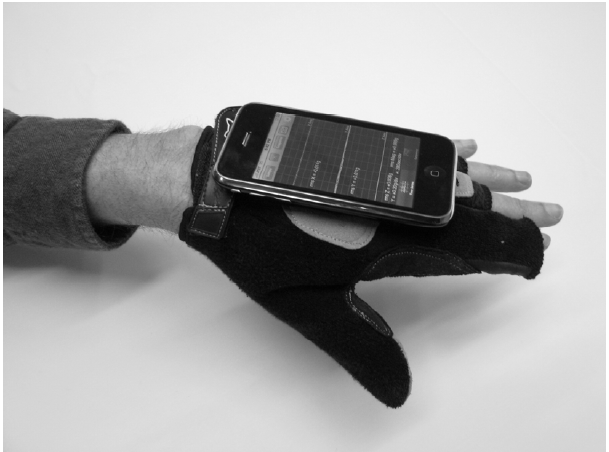
\includegraphics[scale=0.3]{./img/moyne-iphone.png}
  % matrixargseg.png: 296x162 pixel, 100dpi, 7.52x4.11 cm, bb=0 0 213 117
  %\caption{Estágio desenvolvimento de jogos ~\cite{fullerton2008game}}
\caption[Aplicação para \textit{smartphone} com a finalidade de identificar sinais de tremor]{Aplicação para iPhone com a finalidade de identificar sinais de tremor ~\cite{lemoyne2010}}
 %  \caption{Estágio desenvolvimento de jogos}
 \label{fig:iphone-tremor}
\end{figure}


Como apresentado nos trabalhos relacionados, as soluções existentes para~\ac{sms} dos sinais motores utilizam sensores vestíveis (\textit{wearables}), que comumente são incorporados à roupa ou ao corpo do usuário~\cite{classifiersparkinson2014}. De acordo com a perspectiva do usuário, estes sensores são considerados invasivos e estereotipados~\cite{aarhus_negotiating_2010}. Por outro lado, o gerenciamento medicamentoso do~\ac{dp} necessita de um cuidado acurado e diário~\cite{parkself2015,quantitativeparkinson2011}. Por este motivo, é que esta tese pretende prover um mecanismo para quantificar os sinais motores do~\ac{dp} através da indução da execução dos movimentos.


\section{Objetivos}\label{section:objetivos}
Nesta tese, tem-se como objetivo a conceber uma solução computacional que induza o usuário a executar movimentos para avaliação motora. Pretende-se usar jogos eletrônicos como forma de: \textbf{induzir}, \textbf{motivar} e abstrair o monitoramento de dados de saúde de uma maneira \textbf{não invasiva} e longe do \textbf{contexto de tratamento de saúde}.

Nesta tese, foi proposto uma arquitetura de software para o desenvolvimento de jogos eletrônicos integrados a um SMS, onde, demonstrou-se a viabilidade desta arquitetura com a implementação de um jogo capaz de monitorar um sintoma do~\ac{dp}, como estudo de caso.

%Objetivou-se criar um~\ac{sms} integrado à um jogo eletrônico capaz de: induzir a execução de uma avaliação motora que torne possível o processamento dos sinais biomecânicos e consequentemente identificar a presença de sintomas do~\ac{dp}. 

A avaliação da tese foi realizada em duas etapas: na primeira, avaliou-se a capacidade de monitoramento dos indivíduos com \ac{dp} em um estudo analítico de caso-controle; na segunda, avaliou-se a possibilidade de inserir este monitoramento na rotina diária dos pacientes. O estudo analítico de caso-controle, onde foi realizado uma avaliação com 30 sujeitos de pesquisa (15 do grupo controle e 15 diagnosticados com~\ac{dp}). Como resultado, foi identificado e quantificado o sintoma da bradicinesia. Para distinguir os grupos (caso-controle e diagnosticados com~\ac{dp}), utilizamos uma~\ac{svm} para classificação dos dados~\cite{datamining2005}, com a qual obteve-se uma acurácia de 86,66\%. Avaliou-se a adequação da abordagem de monitoramento dos sinais motores na rotina diária usando jogos eletrônicos, aplicando a técnica~\ac{gqm}~\cite{van1999goal}. Nesta avaliação, 90,00\% dos avaliados consideraram a abordagem não-invasiva e incorporável a rotina diária. 

\section{Metodologia}
Esta pesquisa foi submetida à avaliação pelo Comitê de Ética da UFCG (\textbf{CAAE: 14408213.9.1001.5182})~\footnote{Plataforma Brasil, url: http://aplicacao.saude.gov.br/plataformabrasil/} (Apêndice~\ref{sec:comite}), somente depois da aprovação deste é que os dados foram coletados. A metodologia de pesquisa possui aspectos qualitativos e quantitativos. Referente ao aspecto qualitativo, buscou-se identificar a importância desta tese junto à comunidade de especialistas da área de saúde (Seção~\ref{sec:entrevista_semi_estruturada}). Nos aspectos quantitativos, essa pesquisa fez uma análise do sensores de movimento e avaliou a acurácia da aquisição de sinais motores e possibilidade de identificar os sinais do~\ac{dp} baseado na Cinemática Angular do Movimento Humano. Por meio dos dados coletados, pudemos classificar a normalidade e dificuldade na execução de movimentos de abdução e adução dos braços~\cite{mcginnis2013biomechanics}, como será apresentado na Seção~\ref{sec:resultado_svm}. Para avaliar a aceitabilidade da proposta sob a perspectiva do usuário, utilizou-se uma análise~\ac{gqm} a qual é uma abordagem hierárquica que inicia com objetivo principal e o divide em questões mensuráveis~\cite{saraiva2006}, como será apresentado na Seção~\ref{gqm_usuarios}.

Em resumo, três questões foram utilizadas como base para a definição da metodologia do trabalho em três diferentes etapas sequenciais:
	\begin{description}
	\item[QUESTÃO 1] Quais os benefícios de acompanhar os sinais motores do paciente diariamente, do ponto de vista do profissional da saúde?
	\item[QUESTÃO 2] Como melhor adquirir e quantificar sinais motores utilizando sensores de movimento para monitorar os sinais de \ac{dp}?
	\item[QUESTÃO 3] Na perspectiva dos usuários, a abordagem de quantificar os sinais motores é considerada não-invasiva e aplicável à rotina diária?
	\end{description}

As seguintes atividades foram realizadas para a execução do trabalho:

\begin{enumerate}

\item{Realizar revisão bibliográfica e coleta de requisitos junto a profissionais de saúde.}

\item{Definir o conceito da abordagem, denominada \ac{jogue-me}, baseada em captura de sinais motores através de sensores de movimento, utilizando jogos eletrônicos e processamento dos sinais para transformá-los em informações de saúde.}


\item{Analisar a perspectiva dos profissionais de saúde em relação ao acompanhamento dos sinais motores dos pacientes com~\ac{dp} (os profissionais foram indagados sobre a melhora na tomada de decisão quanto ao acompanhamento dos sinais) e verificar se os parâmetros motores, como velocidade angular e amplitude do movimento dos braços, são importantes para realizar o acompanhamento dos sinais do~\ac{dp}. Procurou-se encontrar, junto ao profissional de saúde, a importância do monitoramento dos sinais motores e os benefícios trazidos por este, através de uma abordagem de pesquisa qualitativa. Com esta pesquisa, foi possível validar a \textbf{QUESTÃO 1}, que consiste em verificar a importância do acompanhamento de sinais motores integrados à rotina diária do paciente.}

\item{Validar o uso de sensores para classificação dos dados através do processamento dos sinais motores adquiridos por sensores de movimento utilizados em jogos eletrônicos. A classificação consistiu em aplicar os sinais numa~\ac{svm} para distinguir indivíduos do grupo controle ante indivíduos diagnosticados com~\ac{dp}.
O resultado dessa pesquisa demonstrou a viabilidade da abordagem e, consequentemente, validou a \textbf{QUESTÃO 2} do trabalho.}

\item{Definir a arquitetura de software que viabilizou tecnicamente a abordagem~\ac{jogue-me}. Nesta pesquisa, definimos um arcabouço de software para encapsular o desenvolvimento de jogos com essa abordagem.}

\item{Validar a solução~\ac{jogue-me} do ponto de vista computacional. A solução foi validada através da implementação da arquitetura e do desenvolvimento de jogos. Com esta etapa, demonstrou-se ser possível realizar monitoramento de dados motores de forma não invasiva, ou seja, sem os jogadores perceberem que estão fornecendo dados de saúde.}

\item{Verificar junto ao público alvo (portadores de~\ac{dp}) os requisitos de usabilidade, adequação à rotina diária, segurança física e se a proposta é considerada invasiva na perspectiva do paciente. Com esta avaliação, avaliou-se a \textbf{QUESTÃO 3} da pesquisa.}

\end{enumerate}

\subsection{Termo de Consentimento Livre e Esclarecido (TCLE)}
Antes da realização da coleta dos dados, expomos aos sujeitos da pesquisa as informações necessárias para a realização do estudo. Desta maneira, o indivíduo consentiu com sua participação através da assinatura do Termo de Consentimento Livre e Esclarecido~\footnote{Resolução Nº 196/96, do Conselho Nacional de Saúde, do Ministério da Saúde (CNS/MS).} (Apêndice~\ref{sec:comite}). 

\subsection{Relação Risco Benefício da Pesquisa}
Os riscos inerentes podem decorrer da exposição de dados dos participantes da pesquisa, o que pode acarretar danos morais e/ou psicológicos. Por esse motivo, foram tomados todos os cuidados para que a identidade do indivíduo não fosse revelada, garantindo assim, privacidade e confidência das informações. Todos os dados coletados, estão disponibilizados para pesquisa futura, permitindo o uso para pesquisa a todas instituições envolvidas (UFCG, UFAL e IFAL). No entanto, preservamos a identidade dos participantes da pesquisa e omitimos todos os dados que permitissem sua identificação, conforme descrito no Termo de Consentimento Livre e Esclarecido.

Durante a realização da pesquisa com os participantes da pesquisa, houve uma preocupação referente a possíveis constrangimentos por parte do sujeito da pesquisa. Caso, não conseguisse realizar a pesquisa ou responder alguma pergunta devido ao comprometimento da doença. O pesquisador prestou total assistência, orientando-os adequadamente. Mas, salienta-se que os riscos apresentados justificam-se pelo benefício de monitorar os sinais do~\ac{dp} para um melhor tratamento da doença.


\subsection{Confidencialidade}
Os dados do estudo em questão são considerados propriedade conjunta das partes envolvidas (UFCG, UFAL e IFAL). Porém, sua utilização por terceiros necessita de prévia autorização de todos. No entanto, na submissão do Projeto ao Comitê de Ética da UFCG (\textbf{CAAE: 14408213.9.1001.5182}), expressou-se o comprometimento em tornar público os resultados da pesquisa, sejam estes favoráveis ou não.


\section{Contribuições}
Nas últimas décadas, o monitoramento e quantificação dos sinais motores têm sido objeto de pesquisa recorrente na computação, eletrônica, bioinformática e saúde~\cite{reviewassesenspark2015}. As pesquisas nessa áreas, são fundamentais para a compreensão do progresso de doenças crônicas como o~\ac{dp} e também para auxiliar os médicos no acompanhamento de seus pacientes.

Nesta tese, foi desenvolvida uma arquitetura de software (Capítulo~\ref{arquitetura_captura}) que permite: quantificar, avaliar e identificar o sintoma de bradicinesia do~\ac{dp} induzindo o usuário a executar movimentos de avaliação motora, de uma forma lúdica e integrada a um jogo eletrônico, e longe do contexto de tratamento da saúde.

Do ponto de vista clínico, tornou-se possível identificar como está a saúde do paciente e em que momento o tratamento medicamentoso é eficaz. Atualmente, um detalhamento das flutuações motoras do~\ac{dp} é realizado por auto-relatórios em avaliações diárias dos pacientes que informam em que período do dia a medicação está surtindo efeito~\cite{reviewassesenspark2015}. No entanto, para uma avaliação dos sintomas motores mais acurado, é necessário poder induzir a execução de movimentos para avaliação motora de modo a mensurar quantitativamente os sintomas do~\ac{dp}~\cite{wiiassesspark2016}.

Por estes argumentos apresentados, foi desenvolvido nesta tese um mecanismo quantitativo de avaliação da eficácia do tratamento que utiliza um jogo eletrônico que induz o usuário a executar movimentos de avaliação motora de uma maneira não-invasiva. Esta abordagem de monitoramento, resulta em benefícios aos médicos para um tratamento mais efetivo e acurado da dosagem medicamentosa. Os resultados obtidos, com arquitetura de software desenvolvida, permitiu identificar e estimar a gravidade do sintoma da bradicinesia e das complicações motoras mensuradas num estudo de caso-controle, e isto é um resultado bastante relevante para esta tese.

Como possível cenário de uso da pesquisa, supondo que um paciente de uma doença crônica como o~\ac{dp} faz uso de medicamento antiparkinsoniano e possui um jogo de monitoramento de sinais do~\ac{dp} em sua residência, caso ele utilize o jogo em diferentes momentos do dia, os sinais podem ser quantificados sem a presença de um profissional de saúde, que poderia visualizar a melhora ou piora do estado de saúde do seu paciente ao longo dos dias. A partir da presente abordagem, o médico, ao possuir a informação, poderia gerenciar melhor a dosagem medicamentosa e, consequentemente, prolongar a qualidade de vida do paciente~\cite{abn2010}.

%
%Atualmente, os jogos são aplicados para melhora da saúde em diferentes contextos. No entanto, nenhum dos trabalhos relacionados pretendem identificar sinais para monitorar o estado de saúde. Logo, este trabalho visa desenvolver um ambiente de jogo que motive a execução de movimentos específicos, com o propósito de quantificar os sinais motores dos usuários.
%
%No entanto, alinhar a jogabilidade e a capacidade de monitoramento dos sinais de saúde não é trivial, pois deve ser levado em consideração o uso dos sensores e deve-se definir quais movimentos ou ações permitem a identificação dos sinais motores. Por este motivo, a proposta de um~\ac{sms} dos sinais motores usando jogos necessita de um acompanhamento de um profissional de saúde para supervisionar e auxiliar nas definições dos movimentos e ações dos usuários. 

%Posteriormente, na posse dessas ações, deverá ser testada a execução dessas atividades e sua aquisição para uma possível classificação dos dados conforme proposto nesta tese.
%os trabalhos já existentes~\cite{Ballegaard:2008:HEL:1357054.1357336,patel_monitoring_2009,visionbased2009,bachlin_parkinsons_2009,albanese2012}.
%De posse dos movimentos e da captura dos dados será feito um levantamento de um \textit{game design} que permita executar os movimentos em  um ambiente lúdico e divertido como um jogo para entretenimento ~\cite{sweetser2005-gameflow}.



\section{Organização do Documento}
O restante deste documento está organizado da seguinte forma:
\begin{itemize}
	\item No Capítulo~\ref{chapter:fundamentacao} está descrita a fundamentação teórica relacionada ao trabalho.
	\item No Capítulo~\ref{chapter:abordagem_gahme} está definida a abordagem \ac{jogue-me} para indução e monitoramento dos sinais motores de maneira não invasiva usando jogos eletrônicos.
	\item No Capítulo~\ref{chapter:arquitetura_captura} é apresentada a arquitetura de software da abordagem.
	\item No Capítulo~\ref{chap:avaliacao} são apresentados os experimentos realizados para avaliar a tese.
	\item No Capítulo~\ref{chapter:conclusoes_futuros} são apresentadas as conclusões do trabalho e propostos trabalhos futuros.
\end{itemize}
